% !TeX encoding = UTF-8
\documentclass[12pt,ngerman,a4paper,parskip]{scrartcl}
\usepackage[utf8]{inputenc}
\usepackage[T1]{fontenc}
\usepackage[ngerman]{babel}
\usepackage[a4paper,left=2cm,right=2cm,top=3cm,bottom=3cm]{geometry}
\usepackage{svg}
\usepackage[hidelinks]{hyperref}

% Code listings
\usepackage{minted}

% Make the frame parameter available to includegraphics
\usepackage[export]{adjustbox}

% Use helvetica font
\usepackage{helvet}
\renewcommand{\familydefault}{\sfdefault}

% Format header and footer
\usepackage{fancyhdr}
\pagestyle{fancy}
\fancyhf{} 
\fancyfoot[R]{\thepage}
\fancyhead[L]{\small GPT Partitionstabellen - Nikos Epping}

% Setup quotes
\usepackage{csquotes}
\MakeOuterQuote{"}

% Remove trailing periods from section numbers
\renewcommand{\autodot}{}

\begin{document}

% No page numbers yet
\pagenumbering{gobble}

\begin{titlepage}
    \begin{center}
        \vspace*{1cm}

        \small {\textbf{ENTWURF}}
            
        \Huge
        \textbf{GPT Partitionstabellen}
            
        \vspace{1cm}
            
        \Large
        \textbf{Nikos Epping}
            
   		\vspace{0.8cm}
            
        Seminararbeit
        
        \large 
        Algorithmen und Datenstrukturen

        Wintersemester 2020/21

        \vspace{2cm}

        \begin{center}
        \begin{tabular}{ p{2.5cm} l }
            \textbf{Prüfer} & Prof. Dr. Martin Guddat \\
            \textbf{Abgabe} & 16.12.2020
            \end{tabular}
        \end{center}

        \vfill
            
        \includesvg[width=0.4\textwidth]{content/graphics/whs-logo.svg}
            
    \end{center}
\end{titlepage}


\newpage

\tableofcontents

\newpage

% Start page numbering here
\pagenumbering{arabic}

\section{Einleitung}
Die Speicherung von Daten auf einem Datenträger kann auf zahlreiche unterschiedliche Varianten realisiert werden.
Verschiedene Dateisysteme ordnen die gleichen Daten unterschiedlich auf einem Datenträger an.
Beispielsweise unterteilt das Dateisystem \textit{ext2} Dateien in Blöcke und verwaltet diese mit sogenannten \textit{inodes}, wohingegen bei \textit{Btrfs} die Blöcke anhand einer Baumstruktur organisiert werden. 
Jede Speicherungsmethode hat Vor- und Nachteile in verschiedenen Anwendungsfällen, weshalb es nützlich sein kann, mehrere verschiedene Dateisysteme auf einem Datenträger zu betreiben.
Dazu wird ein Datenträger in Bereiche unterteilt, die "Partitionen" genannt werden.
Aber auch aus vielen weiteren Gründen kann es hilfreich sein, einen Datenträger in verschiedene Partitionen zu unterteilen.

Damit ein Computersystem die Daten auf einem Datenträger sinnvoll lesen kann, muss eindeutig sein, wie diese gespeichert sind.
Dafür werden Partitionstabellen verwendet, die speichern, welche Partitionen auf einem Datenträger vorliegen.

Ein Standard, der seit den 1980er-Jahren verwendet wird, ist der "Master Boot Record" (MBR).
Dieser besitzt allerdings einige technische Limitationen\footnote{Vgl. Abschnitt \ref{sec:gpt_advantages}}, weshalb eine neue Spezifikation mit dem Namen "GUID Partition Table" (GPT) entwickelt wurde.\cite{drive-partition-limits}
Diese Spezifikation wird in dieser Ausarbeitung genauer erläutert.


\section{Partitionstabellen}
Die Speicherung von Daten auf einem Datenträger kann auf zahlreiche unterschiedliche Varianten realisiert werden.
Verschiedene Dateisysteme ordnen die gleichen Daten unterschiedlich auf einem Datenträger an.
Beispielsweise unterteilt das Dateisystem \textit{ext2} Dateien in Blöcke und verwaltet diese mit sogenannten \textit{inodes}, wohingegen bei \textit{Btrfs} die Blöcke anhand einer Baumstruktur organisiert werden. 
Jede Speicherungsmethode hat Vor- und Nachteile in verschiedenen Anwendungsfällen. Daher kann es nützlich sein, mehrere verschiedene Dateisysteme auf einem Datenträger zu betreiben.
Dazu wird ein Datenträger in Bereiche unterteilt, die \textit{Partitionen} genannt werden.

Partitionstabellen sind Datenstrukturen, die meist zu Beginn\footnote{
    Der "Beginn" bezeichnet hier den Bereich, den ein jeweiliger Datenträger mit LBA 0 (vgl. Abschnitt \ref{sec:addressing:lba}) adressiert.
}
eines Datenträgers vorliegen und Informationen über dessen Partitionen beinhalten.
Dies ist zwingend notwendig, damit ein Computersystem die Daten auf einem Datenträger sinnvoll lesen kann.
Außerdem beinhalten Partitionstabellen üblicherweise den sogenannten \textit{Bootloader}. Dabei handelt es sich um den Code, der ausgeführt wird, wenn ein Computersystem von diesem Datenträger starten soll.

\section{Adressierung}
In Partionstabellen sind, unter anderem, Start und Ende der einzelnen Partitionen gespeichert.
Dafür wird eine Nomenklatur benötigt, um die Bereiche auf dem physischen Datenträger zu adressieren.

\subsection{Cylinder-Head-Sector}
Das Verfahren "Cylinder-Head-Sector" (CHS) orientiert sich am physischen Aufbau von Festplatten.
Durch Kombination von Lesekopf, Sektor und Zylinder / Spur (vgl. Abbildung \ref{fig:chs}) entsteht sozusagen ein dreidimensionales Koordinatensystem, in dem eine Position auf einem Datenträger eindeutig identifiziert werden kann.

\begin{figure}[ht]
    \centering
    \fbox{\includesvg{content/graphics/CHS}}
    \caption{Adressierung dines Datenträgers nach dem CHS-Verfahren}
    \label{fig:chs}
\end{figure}

In modernen Festplatten werden allerdings oft komplexere Geometrien zur Anordnung der Daten verwendet, als von CHS vorgesehen sind.
Diese Geometrien werden in diesen Fällen meist von einem Festplatten-Controller, welcher den tatsächlichen Aufbau der Festplatte kennt, in CHS-Werte übersetzt, um die Daten zu adressieren.\cite{pollard2011}
Außerdem sind modernere Datenträger, wie zum Beispiel Flash-Speicher in SSDs, grundlegend anders aufgebaut als klassische Festplatten.

Daher entspricht die CHS-Adressierung heutzutage nur noch in den seltensten Fällen dem tatsächlichen physischen Aufbau eines Datenträgers. 
Mittlerweile wird CHS als obsolet angesehen und durch LBA\footnote{Siehe Abschnitt \ref{sec:LBA}} ersetzt.


\subsection{Logical Block Addressing}
\label{sec:LBA}
Bei dem Verfahren "Logical Block Addressing" (LBA) werden die Daten auf einem Datenträge in 512 Byte große Blöcke (Sektoren) unterteilt, die aufsteigend nummeriert werden.
Der Controller des Datenträgers, der die genaue Geometrie kennt, übersetzt die Block-Nummer dann in den physischen Speicherort der Daten.


\section{GUIDs}

Wie der Name vermuten lässt, verwendet GPT \textit{GUID}s (Globally Unique Identifier), beispielsweise um Partitionen eindeutig zu identifizieren.
Dabei handelt es sich um 128 Bit große Zahlen, die verwendet werden können, um Informationen eindeutig zu identifizieren.

GUIDs sind allgemeiner als \textit{UUID}s (\textbf{U}niversally \textbf{U}nique \textbf{ID}entifier) bekannt, in dieser Ausarbeitung wird allerdings die Bezeichnung GUID verwendet, um konsistent mit GPT zu sein.

\subsection{Motivation}
Aktuelle Softwaresysteme sind oft Zusammenschlüsse aus verschiedenen Anwendungen oder skalierbare Cloud-Lösungen mit mehreren Knoten / Instanzen.
In diesen Systemen ist es nicht trivial, Informationen eindeutig zu identifizieren. Einfache, aufsteigende IDs sind beispielsweise nicht praktikabel, wenn mehrere Knoten in einem solchen System IDs vergeben können, da so Überschneidungen auftreten können.

Die Synchronisierung der bereits vergebenen IDs zwischen allen Knoten ist aufwändig, fehleranfällig und beeinträchtigt die Skalierbarkeit, wodurch diese Lösung meist nicht verwendet wird.
Auch die Verwendung einer zentralen Registrierungsstelle, die als führendes System IDs vergibt, ist nicht ideal, da so ebenfalls die Skalierbarkeit beeinträchtigt wird und darüberhinaus ein Single Point of Failure geschaffen wird, wodurch der Vorteil eines verteilten Systems wieder zunichte gemacht wird.

GUIDs lösen diese Probleme, da sie als praktisch eindeutig verwendet werden können, ohne dass eine Abstimmung mit anderen Knoten oder eine zentrale Registrierungsstelle notwendig ist.
Kollisionen sind zwar nicht ausgeschlossen, aber so unwahrscheinlich, dass sie in der Praxis nicht berücksichtigt werden müssen.


\subsection{Generierung}
Bei GUIDs wird zwischen 5 Versionen unterschieden, die jeweils unterschiedliche Methoden zur Generierung der 128 Bits verlangen.
Welche Version vorliegt, ist an den höchstwertigsten 4 Bits des siebten Oktetts einer GUID zu erkennen.

Je nach Anwendungsfall können verschiedene Methoden, also GUID-Versionen, besser geeignet sein.
Eine Version wird beispielsweise auf Basis der Systemzeit generiert, während eine andere Variante komplett zufallsbasiert erstellt wird.\footnote{
    Auf die Details der Generierung wird hier nicht weiter eingegangen, das dies den Rahmen dieser Ausarbeitung sprengen würde.
}

\subsection{Darstellung}
Bei einer Darstellung in Textform wird eine GUID in 5 Gruppen unterteilt, die in Tabelle \ref{tbl:guid_layout} aufgeführt sind.

\begin{table}[ht]
    \caption{Aufbau einer GUID der Version 1}
    \label{tbl:guid_layout}

    \begin{center}
        \begin{tabular}{|l|l|}
        \hline
        \textbf{Feld}                                                                                         & \textbf{Größe (Oktette)} \\ \hline
        \texttt{time\_low}                                                                                    & 4                        \\ \hline
        \texttt{time\_mid}                                                                                    & 2                        \\ \hline
        \texttt{time\_hi\_and\_version}                                                                       & 2                        \\ \hline
        \begin{tabular}[c]{@{}l@{}}\texttt{clock\_seq\_hi\_and\_res} \\ \texttt{clock\_seq\_low}\end{tabular} & 2                        \\ \hline
        \texttt{node}                                                                                         & 6                        \\ \hline
        \end{tabular}
    \end{center}
\end{table}

Diese Unterteilung basiert auf den Feldern der ersten, Systemzeit-basierten Version, wird aber bei allen Vesionen in der Darstellung verwendet, weshalb die Bezeichnungen der Felder nur berenzt aussagekräftig sind.\cite{uuid-rfc}
Die einzelnen Oktette (Bytes) werden jeweils als zweistellige Hexadezimalzahl dargestellt und die einzelnen Gruppen durch Bindestriche getrennt.
Eine GUID könnte also zum Beispiel wie folgt aussehen:

\begin{center}
    \texttt{f81d4fae-7dec-11d0-a765-00a0c91e6bf6}
\end{center}


\section{GUID Partition Table}
\label{sec:gpt}
In diesem Abschnitt wird der Standard \textit{GUID Partition Table} (GPT) detailliert beschrieben.
Außerdem werden an relevanten Stellen Vorteile gegenüber dem MBR-Verfahren aufgezeigt.

Im Zuge dieser Ausarbeitung wurde außerdem eine Anwendung entwickelt, um Partitions-Informationen aus einem Datenträger, der nach dem GPT-Verfahren partitioniert ist, auszulesen.
Der komplette Quellcode ist im Github-Repository \textit{Nikos410/simple-gpt-reader}\footnote{\url{https://github.com/Nikos410/simple-gpt-reader}} zu finden.
Diese Anwendung wird im Folgenden als \textit{simple-gpt-reader} bezeichnet.


\subsection{Aufbau}
\label{sec:gpt:structure}

Die einzelnen Datenstrukturen, die auf einem Datenträger vorliegen, der nach dem GPT-Verfahren partitioniert ist, werden im Folgenden genauer erläutert.
Eine mögliche Anordnung dieser Datenstrukturen ist in Abbildung \ref{fig:gpt_layout} grafisch dargestellt.

\begin{figure}[ht]
    \begin{center}
        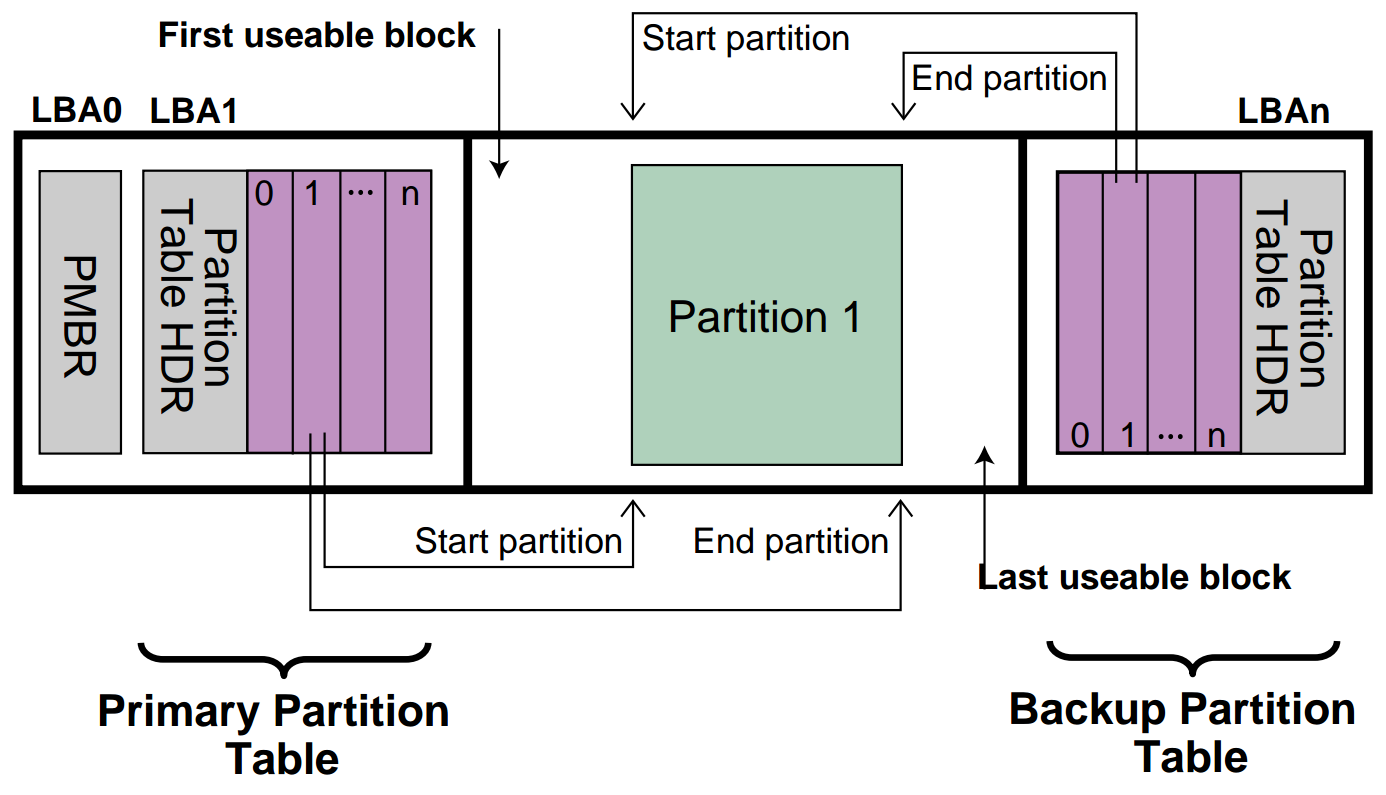
\includegraphics[width=0.6\textwidth]{content/graphics/GPT_Layout.png}
    \end{center}

    \vspace{-0.5cm}

    \caption{Mögliche Anordnungen der Datenstrukturen auf einem Datenträger mit GPT-Partitionierung. \cite{uefi-spec}}
    \label{fig:gpt_layout}
\end{figure}
\vspace{-0.5cm}

\newpage
\subsubsection{Protective MBR}
Viele ältere Betriebssyteme und Programme, die GPT nicht unterstützen, erwarten in LBA 0 einen MBR.
Wenn dieser nicht vorhanden ist, gilt der Datenträger für diese Systeme als nicht oder fehlerhaft partitioniert.
Damit der Datenträger in diesen Fällen nicht überschrieben wird, sieht GPT in LBA 0 einen MBR vor.

Dieser MBR gibt an, dass der Datenträger eine einzelne Partition beinhaltet, die den ganzen Datenträger umfasst.

Dadurch muss in den zuvor erwähnten Systemen üblicherweise ein Nutzer zunächst diese Partitionen explizit löschen, bevor der Datenträger neu partitioniert werden kann.
Da so die GPT-Partitionsdaten sozusagen "geschützt" werden, wird dieser MBR als \textit{Protective MBR} bezeichnet.
Für die Funktion von GPT hat der Protective MBR ansonsten keine Bedeutung.

In Abbildung \ref{fig:protective-mbr} ist der Aufbau eines Datenträgers mit Protective MBR dargestellt.
Es ist zu erkennen dass die \textit{GPT Protective partition} (rot) den gesamten Datenträger umfasst.

\begin{figure}[ht!]
    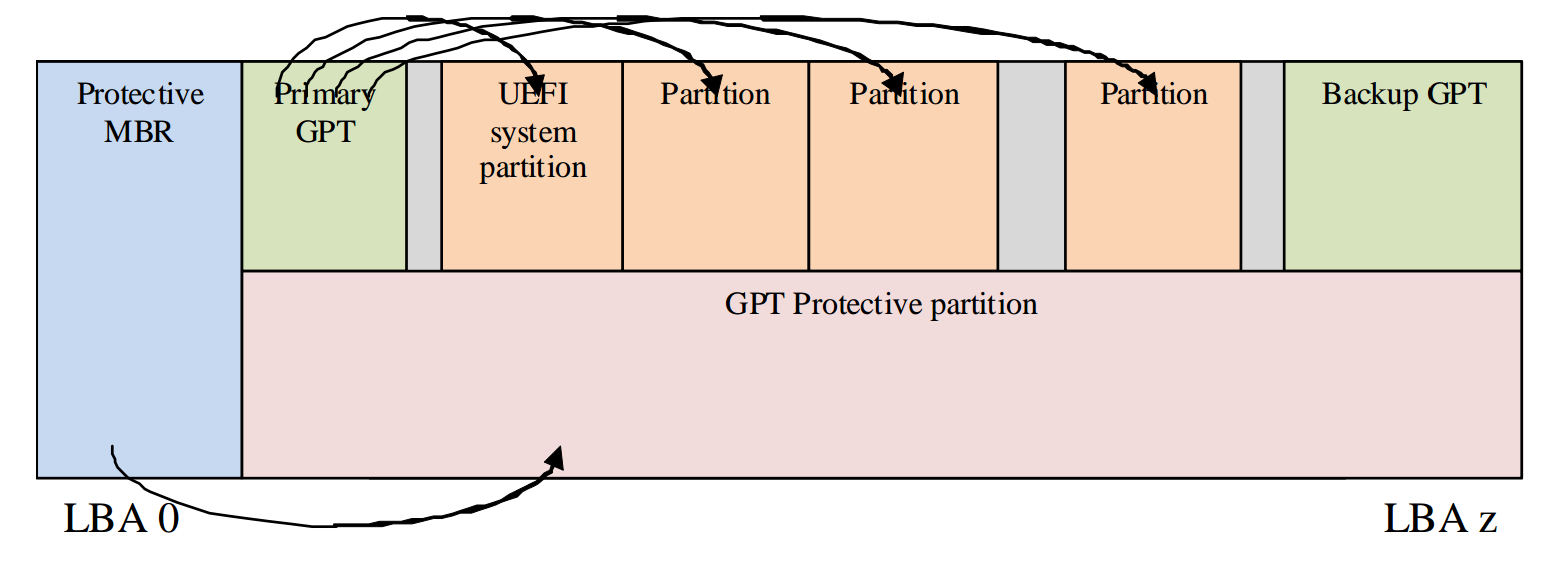
\includegraphics[width=\textwidth]{content/graphics/GPT_Layout_with_protective_MBR.png}
    
    \vspace{-0.2cm}

    \caption{Datenträger mit Protective MBR. \cite{uefi-spec}}
    \label{fig:protective-mbr}
\end{figure}

Bei einem Datenträger, der die maximale von MBR adressierbare Größe überschreitet, beträgt die Größe dieser Partition die maximale Größe, die von MBR adressiert werden kann.
Dadurch belegt diese Partition trotzdem den kompletten von MBR nutzbaren Speicher.
Dieser Fall ist in Abbildung \ref{fig:protective-mbr-large-disk} abgebildet.
Hier ist zu erkennen, dass die \textit{GPT Protective partition} (rot) \textbf{nicht} den gesamten Datenträger umfasst.

\begin{figure}[ht!]
    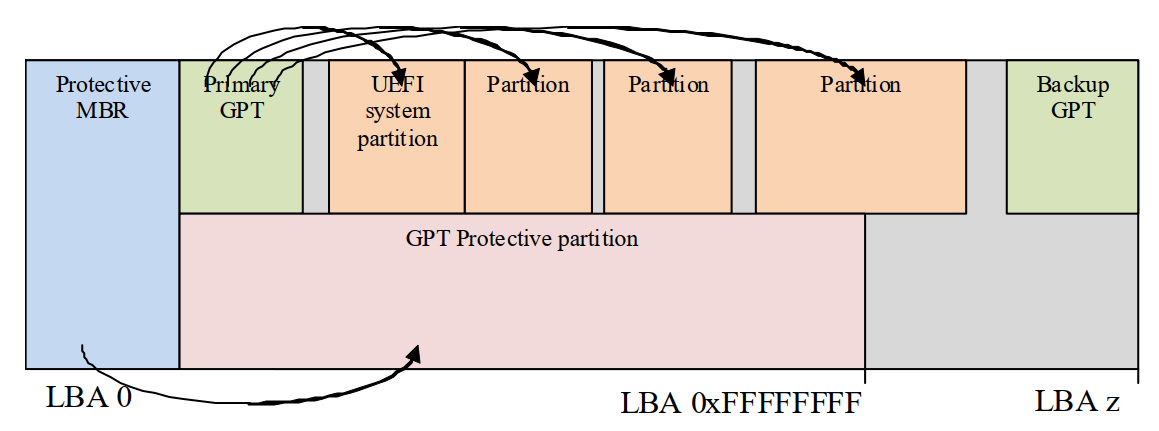
\includegraphics[width=\textwidth]{content/graphics/GPT_Layout_with_protective_MBR_large_disk.png}
    
    \vspace{-0.2cm}

    \caption{Protective MBR auf einem Datenträger, der die maximale von MBR adressierbare Größe überschreitet.\cite{uefi-spec}}
    \label{fig:protective-mbr-large-disk}
\end{figure}


\newpage
\subsubsection{GPT Header}
In LBA 1 befindet sich der sogenannte \textit{GPT Header}.
Dieser Header beinhaltet allgemeine Informationen über den Datenträger.
Im letzten Block eines Datenträgers befindet sich ein zweiter Header, um durch Redundanz Datenverlust vorzubeugen.
Der Header in LBA 1 wird dabei als \textit{primärer}, der Header am Ende als \textit{Backup}-Header bezeichnet.

In Abbildung \ref{fig:GptHeader.hpp} ist die Datenstruktur dargestellt, die im \textit{simple-gpt-reader} verwendet wird, um den Header abzubilden.
Die Bedeutung und der Zweck der einzelnen Felder werden im Folgenden genauer erläutert.

\begin{figure}[ht]
    \inputminted[baselinestretch=1.2, linenos, tabsize=4, breaklines, frame=single]{c++}{content/code/simple-gpt-reader/GptHeader.hpp}
    
    \vspace{-0.5cm}

    \caption{simple-gpt-reader/GptHeader.hpp (Auszug, eigene Darstellung)}
    \label{fig:GptHeader.hpp}
\end{figure}

\begin{itemize}
    \item \textbf{signature}: 
    Das erste Feld beinhaltet eine Signatur, um zu erkennen, ob es sich um einen GPT Header handelt.
    Diese Signatur muss den Wert \texttt{0x5452415020494645}\footnote{
        Dieser Wert entspricht dem ASCII-String "\texttt{EFI PART}"
    } 
    besitzen, damit es sich um einen gültigen GPT Header handelt.

    \item \textbf{revision}:
    Damit der GPT-Standard in Zukunft erweitert werden kann, ist hier die Revision gespeichert, an der man erkennen kann, wie die Daten im Folgenden aufgebaut sind.
    In dieser Ausarbeitung ist die aktuellste\footnote{
        Stand Dezember 2020
    }
    Revision 1.0 beschrieben, in der dieses Feld den Wert \texttt{0x00010000} besitzt.

    \item \textbf{headerSize}:
    Die Größe des Headers in Bytes.
    Üblicherweise entspricht der Wert dieses Feldes der Größe der in Abbildung \ref{fig:GptHeader.hpp} dargestellten Datenstruktur (96 Bytes).
    
    Auch dieses Feld dient dazu, zukünftige Erweiterungen des GPT-Standards, die Änderungen an den Datenstrukturen vornehmen könnten, zu erleichtern.

    \newpage
    \item \textbf{headerCrc32}:
    Die CRC32-Checksumme des Headers.
    Dies dient dazu, die Integrität der Daten sicherzustellen.

    Die Bytes, die für die Berechnung verwendet werden, ergeben sich aus dem Wert des Feldes \textit{headerSize}.
    Es wird diese Anzahl Bytes ab dem Anfang des Headers verwendet.
    Bei der Berechnung wird dieses Feld auf 0 gesetzt, damit der Wert dieses Feldes keinen Einfluss auf die Checksumme hat.
     

    \item \textbf{reserved}:
    Dieses Feld wird nicht verwendet und muss den Wert 0 besitzen. Zukünftige Revisionen können dieses Feld verwenden.

    \item \textbf{myLba}:
    Der Block, in dem sich der aktuelle Header befindet.

    \item \textbf{alternateLba}:
    Der Block, in dem sich der andere Header befindet.
    Beim primären Header verweist dieses Feld auf den Backup-Header, beim Backup-Header auf den primären Header.

    \item \textbf{firstUsableLba}:
    Der erste Block, der für eine Partition verwendet werden kann.
    Üblicherweise ist dies der erste Block nach dem Partitions-Array. (vgl. Abschnitt \ref{sec:gpt:structure:entry-array})

    \item \textbf{lastUsableLba}:
    Der letzte Block, der für eine Partition verwendet werden kann.

    \item \textbf{diskGuid}:
    Eine GUID, die verwendet werden kann, um den Datenträger eindeutig zu identifizieren.\cite{uefi-spec}
    Diese GUID wird beim Anlegen einer GPR-Partitionstabelle erstellt, daher kann eigentlich nur die Partitionstabelle eindeutig identifiziert werden, weshalb die Bezeichnung \textit{diskGuid} irreführend ist.

    \item \textbf{partitionEntryLba}:
    Der erste Block des Partitions-Arrays. 

    \item \textbf{numberOfPartitionEntries}:
    Die Anzahl der Einträge im Partitions-Array.
    Dies entspricht nicht der Anzahl der Partitionen, die tatsächlich auf dem Datenträger vorliegen, sondern der maximalen Anzahl der Partitionen, die im Partitions-Array gespeichert werden können.

    \item \textbf{sizeOfPartitionEntry}:
    Die Größe eines einzelnen Eintrages im Partitions-Array in Bytes.
    Zusammen mit \textit{numberOfPartitionEntries} kann so die Größe des Partitions-Arrays bestimmt werden.

    \item \textbf{partitionEntryArrayCrc32}:
    Die CRC32-Checksumme des Partitions-Arrays.
    
\end{itemize}

Der Rest des LBA-Blocks, in dem sich der Header befindet, muss den Wert 0 besitzen.

\subsubsection{Partitions-Array}
\label{sec:gpt:structure:entry-array}
Im Partitions-Array werden die Informationen zu den einzelnen Partitionen gespeichert.
Auch von dieser Datenstruktur gibt es eine primäre und ein Backup.
Der primäre Header verweist im Feld \textit{partitionEntryLba} auf das primären Partitions-Array, der Backup-Header auf das Backup-Partitions-Array.

In Abbildung \ref{fig:GptPartitionEntry.hpp} ist die Datenstruktur dargestellt, die im \textit{simple-gpt-reader} verwendet wird, um ein Element im Partitions-Array abzubilden.
Die Bedeutung und der Zweck der einzelnen Felder werden im Folgenden genauer erläutert.

\begin{figure}[ht]
    \inputminted[baselinestretch=1.2, linenos, tabsize=4, breaklines, frame=single]{c++}{content/code/simple-gpt-reader/GptPartitionEntry.hpp}
    
    \vspace{-0.5cm}

    \caption{simple-gpt-reader/GptPartitionEntry.hpp (Auszug, eigene Darstellung)}
    \label{fig:GptPartitionEntry.hpp}
\end{figure}

\begin{itemize}
    \item \textbf{partitionTypeGuid}:
    Eine GUID, die den Partitions-Typen identifiziert.
    Damit ist nicht das verwendete Dateisystem gemeint, sondern der Verwendungszweck der Partition.
    Beispielsweise verwendet Linux GUIDs, um zwischen einfachen Daten-Partitionen, RAID-Partitionen oder Swap-Partitionen (Auslagerungsspeicher) zu unterscheiden.
    
    Da GUIDs als global eindeutig angesehen werden können, kann ein Betriebssystem-Hersteller selbstständig neue GUIDs vergeben, ohne diese bei einer zentralen Registrierungsstelle eintragen zu lassen.
    Daher gibt es auch keine vollständige Liste aller existierenden GUIDs, ein Betriebssystem kennt meist nur seine "eigenen" GUIDs.

    \newpage
    Anhand dieses Feldes kann auch erkannt werden, ob dieser Eintrag im Partitions-Array in Verwendung oder leer ist.
    Eine leere GUID\footnote{
        Eine GUID gilt als "leer", wenn alle Felder den Wert 0 besitzen (\texttt{00000000-0000-0000-0000-000000000000})
    } bedeutet, dass dieser Eintrag nicht in Verwendung ist, also keine Partition beschreibt.
    Ein Eintrag, der in Verwendung ist, also eine Partition auf dem Datenträger beschreibt, muss in diesem Feld eine nicht leere GUID besitzen.

    \item \textbf{uniquePartitionGuid}:
    Eine GUID, die diesen Partitions-Eintrag eindeutig identifiziert.
    
    Dies ist ein klarer Vorteil gegenüber dem MBR-Verfahren, bei dem Partitionen meist durch ihre Position auf dem Datenträger identifiziert werden (beispielsweise "Partition 2").
    
    Dort kann es zu Problemen kommen, wenn beispielsweise die erste Partition auf einem Datenträger in 2 Partitionen aufgeteilt wird.
    In diesem Fall erhöht sich entsprechend auch die Partitions-"Nummer" der darauf folgenden Partitionen (beispielsweise wird Partition 2 zu Partition 3).
    
    Die GUID, die von GPT verwendet wird, bleibt hingegen konstant und darf nach dem Anlegen einer Partition nicht mehr verändert werden.

    \item \textbf{startingLba}:
    Der erste Block der Partition, die von diesem Eintrag beschrieben wird.

    \item \textbf{endingLba}:
    Der letzte Block der Partition, die von diesem Eintrag beschrieben wird.

    \newpage
    \item \textbf{attributes}:
    Die einzelnen Bits dieses Feldes entsprechen verschiedenen Attributen.
    Diese Attribute sind für die Partitionierung selbst nicht relevant, sondern spezifizieren vor Allem, wie das Betriebssystem oder die Firmware eines Computers mit dieser Partition interagieren muss.
    Aus diesem Grund wird die Bedeutung der einzelnen Bits hier nicht weiter ausgeführt, da dies auch den Rahmen dieser Ausarbeitung sprengen würde.
    
    \item \textbf{partitionName}:
    Null-terminierter String, der einen Namen der Partition beinhaltet.
    Dieser Name muss nicht dem Namen des Dateisystems, das sich ggf. in dieser Partition befindet, entsprechen.

\end{itemize}

Wenn der Wert des Feldes \textit{sizeOfPartitionEntry} größer ist als die zuvor beschriebene Datenstruktur, muss der Rest des Partitions-Eintrags den Wert 0 besitzen und darf nicht anderweitig verwendet werden.\cite{uefi-spec}

\subsection{Bearbeiten der Partitionstabelle}
Wenn Änderungen an den GPT-Datenstrukturen vorgenommen werden, beispielsweise beim Hinzufügen neuer Partitionen, müssen die folgenden Richtlinien beachtet werden:

\begin{itemize}
    \item Wenn der primäre Header geändert wird, muss auch der Backup-Header entsprechend geändert werden und umgekehrt.
    Dies ist wichtig, damit bei Datenverlust in einem Header der jeweils Andere zur Wiederherstellung verwendet werden kann.

    \item Header und Partitions-Array dürfen in beliebiger Reihenfolge geändert werden.
    
    \item Der Backup-Header muss vor dem primären Header geändert werden.

    \item Nach jeder Änderung an einem Header oder Partitions-Array muss die zugehörige CRC32-Checksumme aktualisiert werden.
    Wenn beispielsweise ein Eintrag im Partitions-Array geändert wird, muss dessen Checksumme (\textit{partitionEntryArrayCrc32}) im Header aktualisiert werden.
    Dadurch wird der Inhalt des Headers geändert, weshalb dessen CRC32-Checksumme (\textit{headerCrc32}) ebenfalls neu berechnet werden muss.
\end{itemize}

\subsection{Gültigkeit prüfen}
Um zu prüfen, ob eine GPT Partitionstabelle gültig ist, müssen folgende Schritte für den primären und sekundären Header durchgeführt werden:

\newpage
\begin{enumerate}
    \item Prüfen, ob das Feld \textit{signature} dem Wert \texttt{0x5452415020494645} entspricht.
    \item Prüfen, ob die CRC32-Checksumme des Headers korrekt ist.
    \item Prüfen, ob sich der Header im Block befindet, der im Feld \textit{myLba} angegeben ist.
    \item Prüfen, ob die CRC32-Checksumme des zugehörigen Partitions-Arrays korrekt ist.
\end{enumerate}

Wenn ein Header fehlerhaft ist, muss geprüft werden, ob der andere Header korrekt ist.
In diesem Fall kann der fehlerhafte Header wiederhergestellt werden, allerdings sollte der Anwender dies explizit bestätigen müssen.\cite{uefi-spec}

\subsection{Bootloader}
\label{sec:gpt:bootloader}

Anders als bei anderen Verfahren besitzt GPT eine spezielle Systempartition, die den Boot-loader-Code beinhaltet.
In dieser Partition können mehrere Einträge hinzugefügt werden, wodurch Multiboot-Systeme deutlich einfacher und vor Allem robuster werden.\cite{heise-mbr-gpt}
Bei einem Datenträger, der kein startbares Betriebssytem beinhaltet, fehlt diese Partition.

Dieser Partitions-Typ besitzt eine fest definierte GUID im Feld \textit{partitionTypeGuid}.
Firmware, die den GPT-Standard unterstützt, muss diese GUID kennen und den Bootloader-Code in dieser Partition ausführen.

Auch dieses Verfahren verbessert die Erweiterbarkeit des GPT-Standards, da die Größe dieser Partition flexibel an die Länge des Bootloader-Codes angepasst werden kann.


\subsection{Limits}
In diesem Abschnitt werden die Grenzen beschrieben, die der GPT-Standard besitzt.

\subsubsection{Maximale Größe eines Datenträgers}
\label{sec:gpt:limits:max-partition-size}

GPT verwendet 64 Bit große Datenstrukturen, um die LBA-Block-Nummern von Anfang und Ende der einzelnen Partitionen zu speichern.
Die üblicherweise verwendete Block-Größe beträgt 512 Bytes, wodurch sich eine maximale verwendbare Größe von $ 2^{64} \cdot 512 \mathrm{B} = 8 \mathrm{ZiB} $ ergibt.\footnote{
    Um diese Größe einzuordnen: Im Jahr 2018 wurde die Datenmenge, die weltweit existierte, auf 33 ZB geschätzt.\cite{global-datasphere-estimate}
}

MBR hingegen verwendet 32 Bit große Datenstrukturen, wodurch sich eine maximale adressierbare Größe von lediglich $ 2^{32} \cdot 512 \mathrm{B} = 2 \mathrm{TiB} $ ergibt.

In den meisten Betriebssystemen entspricht dies auch der maximalen Größe, die ein Datenträger besitzen kann, wenn er nach dem MBR-Verfahren partitioniert ist.
Da MBR allerdings nicht die Block-Nummer des letzten Blockes einer Partition, sondern dessen Länge in Blöcken speichert, können in manchen Betriebssystemen bis zu 4TiB eines Datenträgers verwendet werden. 
Um dies zu erreichen, kann eine 2TiB große Partition angelegt werden, dessen Startblock sich an der größten möglichen LBA-Adresse befindet.
Dieses Verfahren wird allerdings nur von wenigen Betriebssystemen unterstützt, welche intern Block-Nummern verwalten können, die größer als 32 Bit sind.
Diese Betriebssysteme können meist auch das GPT verwenden, weshalb dieses Verfahren in der Praxis selten angewendet wird.\cite{mbr-4tb-workaround}

Für heutige Datenträger sind oft weder 2TiB noch 4TiB ausreichend, weshalb die maximale Kapazität häufig das ausschlaggebenste Kriterium für die Verwendung von GPT ist.

\subsubsection{Maximale Anzahl an Partitionen}
\label{sec:gpt:limits:max-partition-count}

GPT verwendet 32 Bits um die Anzahl der Partitionen auf einem Datenträger zu speichern (\textit{numberOfPartitionEntries}), was bedeutet dass maximal $ 2^{32} $ Partitionen verwaltet werden können.
Dieses Limit wird allerdings nicht von allen Betriebssystemen unterstützt, beispielsweise können unter Linux maximal 256 Partitionen und unter Windows 128 Partitionen auf einem Datenträger verwendet werden.

MBR hingegen kann maximal vier (primäre) Partitionen verwalten.
Um dieses Limit zu erhöhen, können in einer primären Partition weitere logische Partitionen angelegt werden.

\subsection{Vorteile gegenüber MBR}
\label{sec:gpt:advantages}

In den vorherigen Abschnitten wurden viele Vorteile erläutert, die GPT gegenüber MBR besitzt.
Diese Vorteile werden an dieser Stelle noch einmal gesammelt aufgeführt.

\begin{itemize}
    \item \textbf{Maximale Größe von Partitionen:}
    GPT verwendet 64 Bit große Datenstrukturen, um LBA-Block-Nummern zu speichern, MBR 32 Bit.
    Dadurch ergeben sich nutzbare Größen von 8ZiB gegenüber 2TiB (vgl. Abschnitt \ref{sec:gpt:limits:max-partition-size}).

    \item \textbf{Maximale Anzahl von Partitionen:}
    GPT kann $ 2^{32} $, MBR nur 4 primäre Partitionen verwalten (vgl. Abschnitt \ref{sec:gpt:limits:max-partition-count}).

    \item \textbf{Erweiterbarkeit:}
    Die von GPT verwendeten Datenstrukturen sind so konzeptioniert, dass in Zukunft einfach Erweiterungen vorgenommen werden können.
    Beispielsweise werden Revision und Größe der Datenstrukturen in der Partitionstabelle gespeichert (vgl. Abschnitt \ref{sec:gpt:structure}).

    \item \textbf{Datensicherheit:} 
    GPT verwaltet 2 redundante Partitionstabellen in verschiedenen Bereichen eines Datenträgers (vgl. Abschnitt \ref{sec:gpt:structure}).
    
    \item \textbf{Datenintegrität:}
    GPT verwendet CRC32 Checksummen, um die Integrität der Daten sicherzustellen (vgl. Abschnitt \ref{sec:gpt:structure}).

    \item \textbf{Bootloader:}
    GPT besitzt eine spezielle Systempartition, die den Bootloader-Code beinhaltet.
    Dadurch wird die Verwaltung des Bootloader-Codes und die Verwendung von Multiboot-Systemen vereinfacht (vgl. Abschnitt \ref{sec:gpt:bootloader}).

\end{itemize}


\section{Fazit}
TODO



\appendix

\newpage
\section{Glossar}

\textbf{ASCII}:
\textit{American Standard Code for Information Exchange}. Eine weit verbreitete Zeichenkodierung.

\textbf{Auslagerungsspeicher}:
Festplattenspeicher, der als Arbeitsspeicher verwendet werden kann, wenn der eigentliche RAM belegt ist.
Im Englischen auch \textit{swap memory} genannt.

\textbf{Checksumme}:
Ein Wert, der verwendet werden kann, um die Integrität von Daten zu überprüfen.
Im Deutschen auch \textit{Prüfsumme} genannt.

\textbf{CRC}:
\textit{Cyclic Redundancy Check}.
Ein Verfahren, um aus Rohdaten eine Checksumme zu bestimmen.

\textbf{CRC32}:
Eine Variante des \textit{CRC}-Verfahrens, das 32 Bit große Checksummen generiert.

\textbf{Datenintegrität}:
Vollständigkeit, Korrektheit und Unversehrtheit von Daten. 

\textbf{Firmware}:
Sofware, die die Kommunikation zwischen Hardware und Betriebssystem / Anwendungssoftware steuert / ermöglicht.

\textbf{Multiboot-System}:
Ein Computersystem, das verschiedene Betriebssyteme starten kann.

\newpage
\begin{thebibliography}{99}
    \bibitem{ata-5}
        T13 Committee.
        \textit{Information Technology - AT Attachment with Packet Interface - 5 (ATA/ATAPI-5)}.
        Februar 2000.
        \url{https://web.archive.org/web/20110728081430/http://www.t10.org/t13/project/d1321r3-ATA-ATAPI-5.pdf}

    \bibitem{ata-6}
        T13 Committee.
        \textit{Information Technology - AT Attachment with Packet Interface - 6 (ATA/ATAPI-6)}.
        Dezember 2001.
        \url{https://web.archive.org/web/20110728081452/http://www.t10.org/t13/project/d1410r3a-ATA-ATAPI-6.pdf}

    \bibitem{pollard2011}
        Jonathan de Boyne Pollard.
        \textit{The gen on disc partition alignment}.
        \url{http://jdebp.eu/FGA/disc-partition-alignment.html}
        Zuletzt abgerufen am 19.11.2020.

    \bibitem{uuid-rfc}
        P. Leach, Microsoft, M. Mealling, Refactored Networks LLC, R. Salz, DataPower Technology Inc.
        \textit{Request for Comments: 4122 - A Universally Unique IDentifier (UUID) URN Namespace}.
        Juli 2005.
        \url{https://tools.ietf.org/html/rfc4122}

    \bibitem{uefi-spec}
        UEFI Forum.
        \textit{UEFI Specification Version 2.8 (Errata A)}.
        Februar 2020.
        \url{https://www.uefi.org/specifications}

    \bibitem{mbr-4tb-workaround}
        Rod Smith.
        \textit{Working Around MBR's Limitations}.
        \url{http://www.rodsbooks.com/gdisk/workarounds.html}
        Zuletzt abgerufen am 21.11.2020.

    \bibitem{drive-partition-limits}
        UEFI Forum.
        \textit{FAQ: Drive Partition Limits}.
        2010.
        \url{https://www.uefi.org/sites/default/files/resources/UEFI_Drive_Partition_Limits_Fact_Sheet.pdf}


    \bibitem{linux-kernel-genhd}
        Linux kernel developers.
        \textit{genhd.h}.
        \url{https://git.kernel.org/pub/scm/linux/kernel/git/efi/efi.git/tree/include/linux/genhd.h}
        Zuletzt abgerufen am 10.12.2020.

    \bibitem{windows-gpt}
        Microsoft.
        \textit{Windows and GPT FAQ}.
        \url{https://docs.microsoft.com/en-us/windows-hardware/manufacture/desktop/windows-and-gpt-faq}
        Zuletzt abgerufen am 10.12.2020.

    \bibitem{heise-mbr-gpt}
        Mirco Lang, Heise.
        \textit{Festplatten-Partitionen: MBR oder GPT? Tipps \& Tricks.}
        \url{https://www.heise.de/tipps-tricks/Festplatten-Partitionen-MBR-oder-GPT-4351715.html}
        Zuletzt abgerufen am 12.12.2020.

    \bibitem{wikipedia-crc}
        Wikipedia.
        \textit{Cyclic redundancy check}
        \url{https://en.wikipedia.org/wiki/Cyclic_redundancy_check}
        Zuletzt abgerufen am 13.12.2020.
\end{thebibliography}


\section{Abbildungsverzeichnis}
\vspace{-2cm}
\renewcommand{\listfigurename}{}
\listoffigures

\section{Tabellenverzeichnis}
\vspace{-2cm}
\renewcommand{\listtablename}{}
\listoftables

\section{Änderungshistorie}

\textbf{Änderungen in der Endfassung vom 13.01.2021:}

\begin{itemize}
    \item Hinweis, dass ein Partitions-Array mindestens 16 KB groß sein muss, hinzugefügt.

    \item Punkte am Ende von Überschrifts-Nummern entfernt.

    \item Information über Endianess der GPT Datenstrukturen hinzugefügt.
    
    \item Alle Anhänge nummeriert und ins Inhaltsverzeichnis aufgenommen.
\end{itemize}


\newpage
\section{Eidesstattliche Erklärung}
Ich erkläre, dass ich alle Quellen, die ich zur Erstellung dieser Arbeit verwendet habe, im Quellenverzeichnis aufgeführt habe und dass ich alle Stellen, an denen Informationen (Texte, Bilder) aus diesen Quellen in meine Arbeit eingeflossen sind, als Zitate mit Quellenangabe kenntlich gemacht habe.
Mir ist bewusst, dass ein Verstoß gegen diese Regeln zum Ausschluss aus dem Seminar führt.

\vspace{1.5cm}

\small
Bocholt, den 12.01.2021

\vspace{0.8cm}

--------------------------------------------------------\\
Nikos Epping

\end{document}
